\section{From Simulation to a Radio}
\label{sec:cport_sdr}

The demonstration apps talk to a \emph{driver} over a socket rather than
to hardware, which turns out to be the right seam for real radio: an SDR
driver (\texttt{demoapp/sdr\_driver.py}) presenting the same devices puts
the entire C stack on the air with nothing in \texttt{cport/} changed.
It reproduces the SSB model of Section~\ref{sec:rf} sample by sample ---
audio $\rightarrow$ analytic signal (the receiver's own 63-tap Hilbert
design) $\rightarrow$ interpolation to the SDR rate $\rightarrow$ I/Q,
and back, where taking the real part of the decimated baseband
\emph{is} a product detector.  Tuning the radio to the suppressed
carrier makes the two stations' LO error appear as exactly the
audio-band CFO the modem already tracks.  The DSP costs 4.4\,\% of one
core to transmit and 3.1\,\% to receive per audio-second at 2.4\,Msps,
so a laptop runs it comfortably in real time.

Figure~\ref{fig:sdr_setup_loopback} shows the arrangement that needs no
radio at all: the driver cross-connects two stations through the entire
SSB chain --- Hilbert transform, interpolation, int8 quantisation,
decimation and product detection --- so every line of the signal path is
exercised, and the console apps above it cannot tell the difference.
That is what the regression test uses.

\begin{figure}[H]
    \centering
    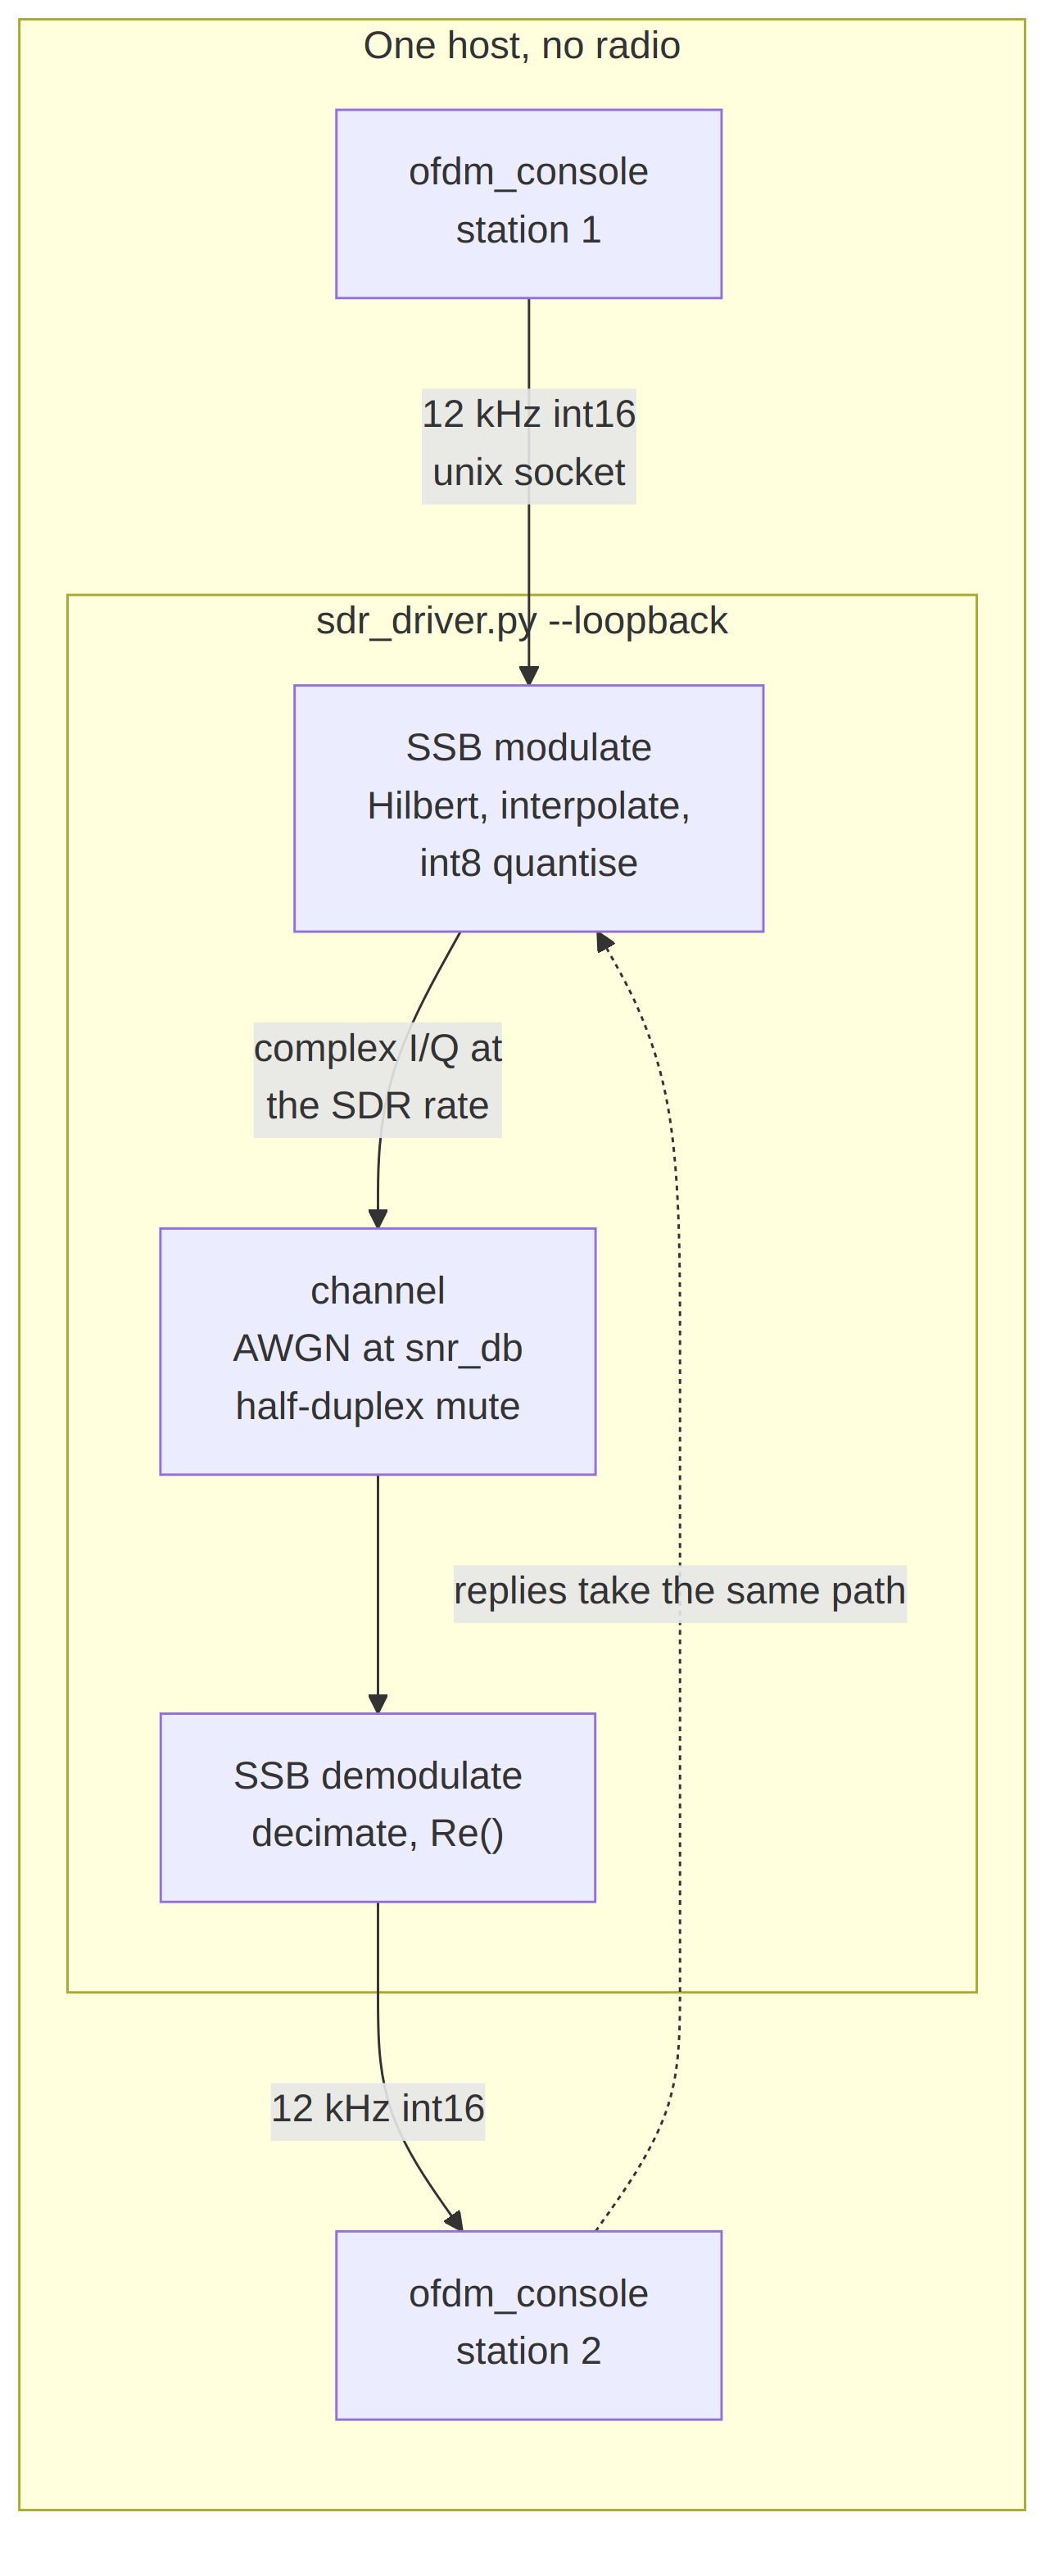
\includegraphics[width=\textwidth]{images/sdr_setup_loopback.png}
    \caption{Hardware-free loopback: two stations cross-connected
             through the full SSB modulation and demodulation chain.}
    \label{fig:sdr_setup_loopback}
\end{figure}

Bringing this up on a HackRF One produced four corrections that no
amount of loopback testing would have found: the local oscillator must
be \emph{offset tuned} (with it on the carrier, the DC leakage lands
inside the 3.5\,kHz passband and the recovered audio was 98\,\% DC ---
the device has neither hardware DC correction nor AGC); the aggregate
gain control is inert and the LNA/VGA/AMP stages must be driven
individually (worth 32\,dB of working level); \texttt{writeStream} only
\emph{queues} samples, so switching back to receive when it returns
truncated the tail of every frame; and a killed process left the radio
\emph{keyed} until a receive stream was opened.

\subsection{Instrumented Measurements}

The measurements of this section share the arrangement of
Figure~\ref{fig:sdr_setup_analyzer}: a tinySA Ultra on USB, used in
both directions.  As an analyser it measures what the radio transmits
--- the spectrum and the drive sweep below; as a source, through its
calibration output (a reference tone at a documented level), it
measures what the receiver makes of a known input --- the receive-chain
calibration reported with the link budget in
Section~\ref{sec:link_budget_measured}.  All are scripted, so the
numbers are reproducible rather than read off a screen.

\begin{figure}[H]
    \centering
    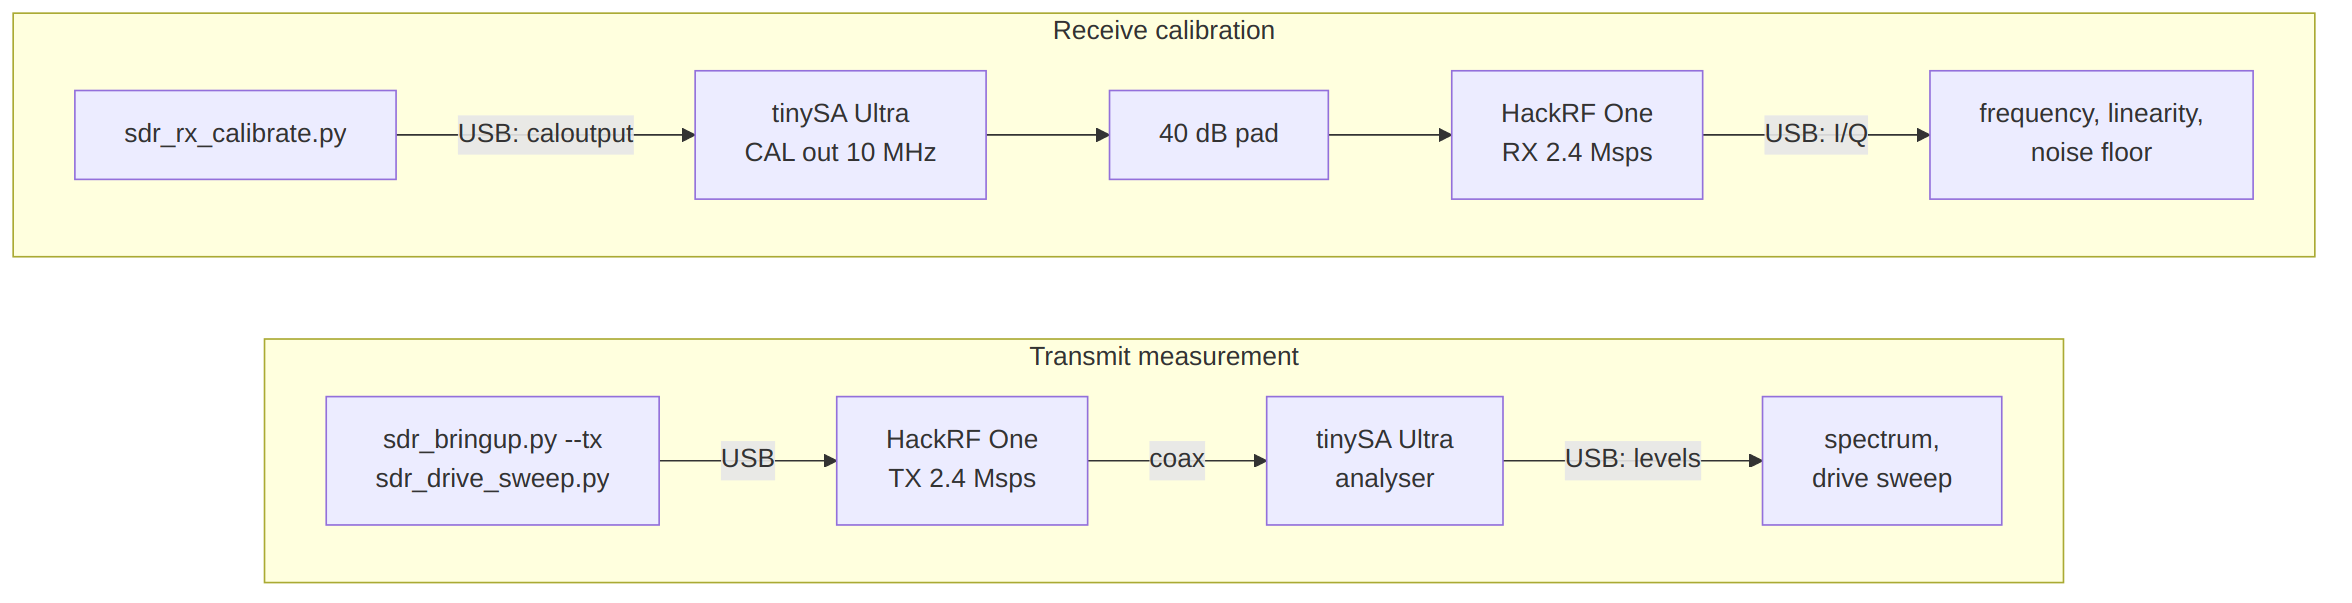
\includegraphics[width=\textwidth]{images/sdr_setup_analyzer.png}
    \caption{Instrumented bench, both directions: as an analyser the
             tinySA measures what the radio transmits; as a source its
             calibration output drives the receiver through a 40\,dB
             pad.}
    \label{fig:sdr_setup_analyzer}
\end{figure}

\subsection{The Transmitted Spectrum}

Figure~\ref{fig:sdr_tx_spectrum} is the waveform measured on a tinySA
Ultra wired to the antenna port, captured by
\texttt{demoapp/tinysa.py} (which sweeps with the transmitter off,
keys it, and max-holds several sweeps).  The occupied band matches the
design: a $-3$\,dB width of 2.42\,kHz against the 2.1\,kHz the
numerology predicts, once the 3\,kHz resolution bandwidth is allowed
for, sitting exactly where the carrier and 300--2400\,Hz audio band put
it.  That single measurement validates the absolute tuning, the
offset-tuning arithmetic, the drive scaling into the 8-bit DAC and the
single-sideband modulation at once --- an error in any of them shows up
as splatter or a mirror image.  Visible 50\,kHz below the signal is the
LO leakage at $-35$\,dBc, the price of the offset tuning that keeps DC
out of the \emph{receive} passband.

\begin{figure}[H]
    \centering
    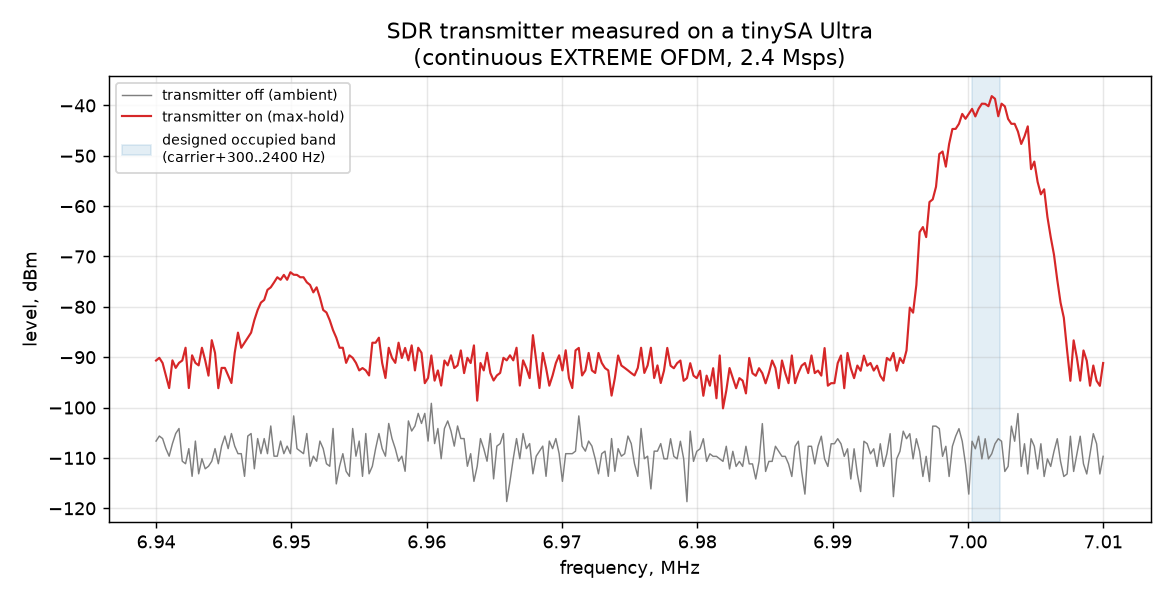
\includegraphics[width=0.92\textwidth]{images/sdr_tx_spectrum.png}
    \caption{The transmitter measured on a tinySA Ultra: continuous
             EXTREME OFDM at 2.4\,Msps, carrier 7.000\,MHz, 3\,kHz RBW.
             The shaded band is the designed occupancy
             (carrier\,$+$\,300\ldots2400\,Hz); the spur at 6.95\,MHz is
             the offset-tuned local oscillator.}
    \label{fig:sdr_tx_spectrum}
\end{figure}

\subsection{How Hard the Radio Can Be Driven}

Figure~\ref{fig:sdr_drive_sweep} sweeps the transmit gain and measures,
at each step, the fundamental, the shoulders 5--10\,kHz outside the
occupied band, and the harmonics.  It should be read from the middle
outwards: below VGA 16 the reported shoulders are the \emph{analyser's}
noise floor rather than the transmitter's, because the fundamental is
only $-58$\,dBm.  Above VGA 32 the degradation is real compression,
provoked by the waveform's $\approx$8\,dB PAPR --- at full drive the
shoulders reach $-22$\,dBc and the second harmonic $-38$\,dBc, both
worse than the $-43$\,dBc usually demanded of spurious emissions.

The asymmetry between the two impairments is the practical result: a
low-pass filter removes the harmonics but does nothing about the
shoulders, which are spectral regrowth a few kilohertz from the carrier
and inside any filter's passband.  The usable window with this waveform
is therefore about VGA 16--32, i.e.\ $-42$ to $-24$\,dBm, and real power
has to come from a \emph{linear} external amplifier rather than from
winding this one up --- the same linearity requirement the OFDM
waveform imposes everywhere else in the chain.

\begin{figure}[H]
    \centering
    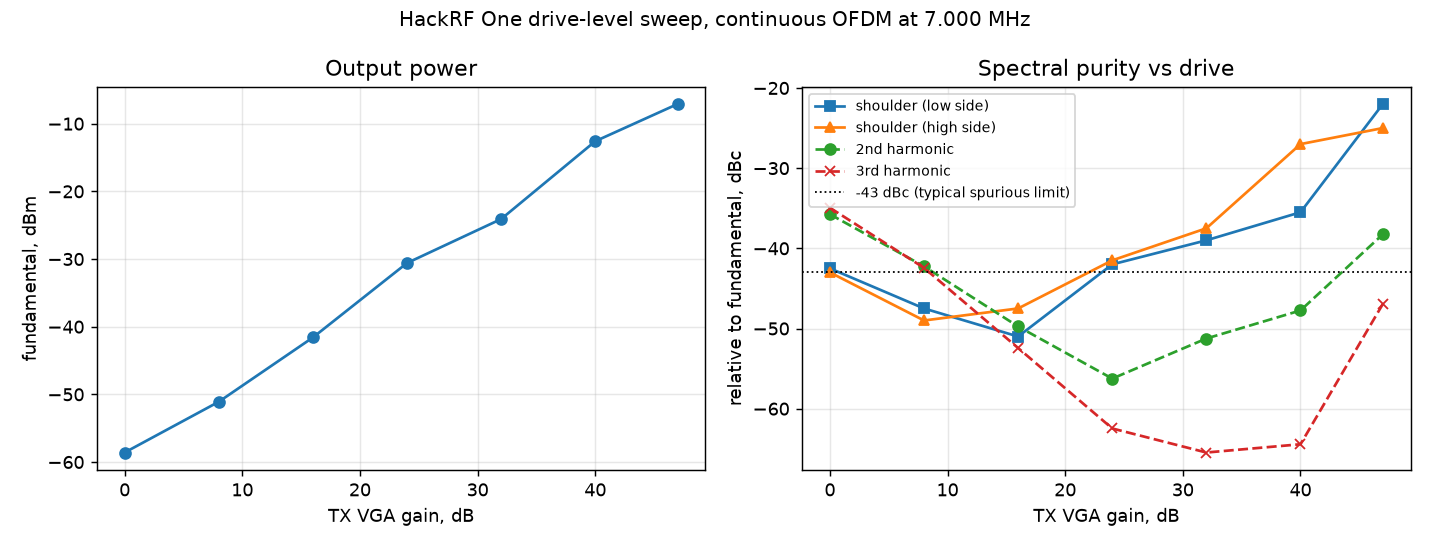
\includegraphics[width=\textwidth]{images/sdr_drive_sweep.png}
    \caption{Drive-level sweep on the HackRF One
             (\texttt{demoapp/sdr\_drive\_sweep.py}): output power, and
             spectral purity relative to the fundamental, against
             transmit gain.  Points below VGA 16 are limited by the
             analyser's noise floor, not by the transmitter.}
    \label{fig:sdr_drive_sweep}
\end{figure}

\subsection{Decoding Off the Air}

A half-duplex radio cannot receive its own transmission, so the last
question --- does a receiver actually \emph{decode} this over a real RF
path? --- needs a separate transmitter.  Figure~\ref{fig:sdr_setup_ammod}
shows the one used: a laptop's sound card plays a generated file into an
AM modulator carried by an external generator at 7.000\,MHz, and the
result reaches the SDR through a 40\,dB pad.

AM demands a different detector, for a reason worth stating because it
is a property of the waveform rather than an inconvenience.  The
receiver is single-sideband: it tunes to a \emph{suppressed} carrier and
takes the real part of the baseband.  Present it with a double-sideband
signal and the lower sideband folds onto the upper one; worse, any
frequency error between the generator and the SDR multiplies the audio
by a slow cosine, splitting every subcarrier in two.  The test therefore
recovers the carrier that AM conveniently provides, derotates by it so
the carrier sits at exactly 0\,Hz and zero phase, and only then takes
the real part.  That is classical synchronous detection, and it is why
the decoded CFO in Table~\ref{tab:offair} reads zero: the carrier lock
has already absorbed the error the modem would otherwise estimate.

\begin{figure}[H]
    \centering
    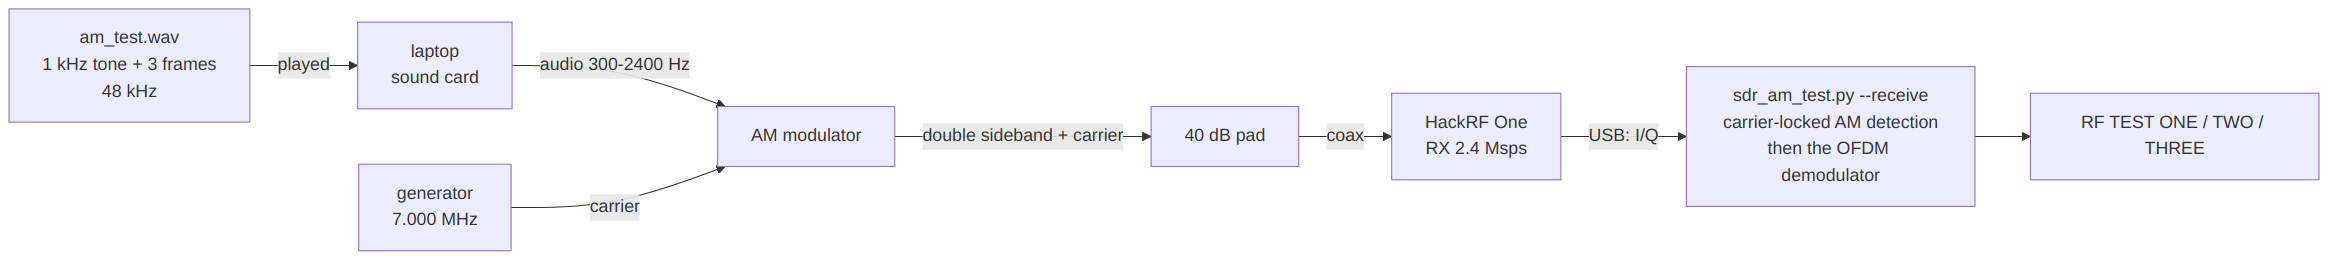
\includegraphics[width=\textwidth]{images/sdr_setup_ammod.png}
    \caption{Off-air receive test: an external AM transmitter feeds the
             SDR through a 40\,dB pad.}
    \label{fig:sdr_setup_ammod}
\end{figure}

\begin{table}[H]
    \centering
    \caption{All three transmitted frames recovered over a 7\,MHz RF
             path (\texttt{results/am\_rx\_offair.wav}).}
    \label{tab:offair}
    \small
    \begin{tabular}{@{}llrr@{}}
    \toprule
    \textbf{Frame} & \textbf{Payload} & \textbf{Length} &
    \textbf{SNR} \\
    \midrule
    NORMAL QPSK 1/2 & \texttt{RF TEST ONE}   & 1.0\,s & $+13.6$\,dB \\
    NORMAL BPSK 1/3 & \texttt{RF TEST TWO}   & 1.8\,s & $+14.4$\,dB \\
    ROBUST BPSK 1/3 & \texttt{RF TEST THREE} & 7.3\,s & $+8.5$\,dB \\
    \bottomrule
    \end{tabular}
\end{table}

Figure~\ref{fig:sdr_waterfall} shows those frames as the demodulator
received them.  The analysis FFT is 128 bins at 12\,kHz, exactly the
modem's own subcarrier grid, so each row is one OFDM bin and the frame
structure of Section~\ref{sec:phy} is directly legible: the Newman tone
comb lighting only a few bins, the Zadoff--Chu symbol closing the
preamble, then the header and the data block filling 300--2400\,Hz.
The spans above each waterfall are computed rather than fitted --- from
the mode's tone-field geometry and the decoded header's own modulation,
code rate and length --- and they land on the measured burst to within
15\,ms.  The comb's end is measurable independently: bin occupancy sits
at 0.17 through the tone fields and jumps to 0.9 at 0.321\,s, against a
predicted 0.320\,s.  It is worth noting that the ZC symbol occupies all
23 carriers, so on a waterfall it resembles data even though it belongs
to the preamble --- which is why it is drawn as its own span.

\begin{figure}[H]
    \centering
    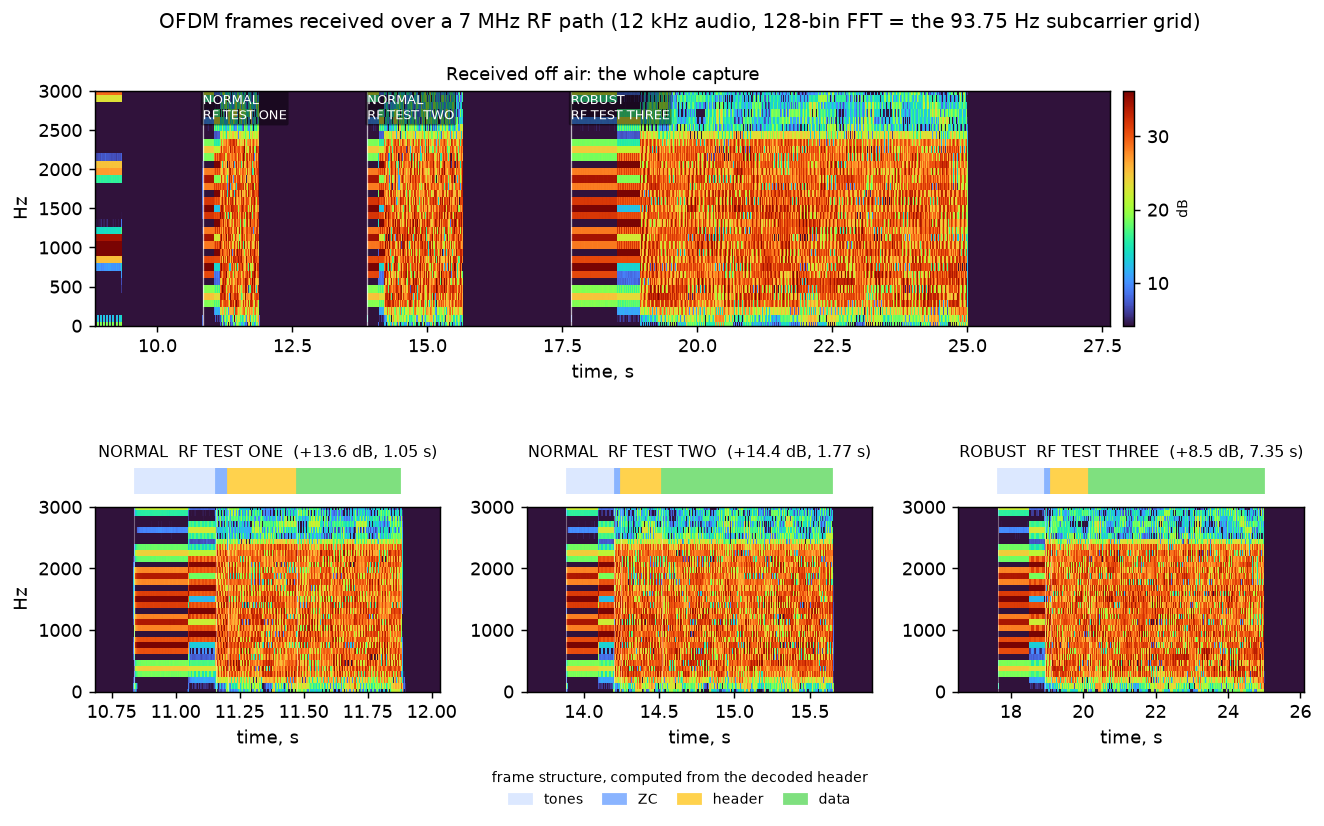
\includegraphics[width=\textwidth]{images/sdr_waterfall.png}
    \caption{Frames received over the air
             (\texttt{demoapp/sdr\_waterfall.py} on
             \texttt{results/am\_rx\_offair.wav}): the whole capture
             above, each frame below with its measured structure.  The
             ROBUST frame carries the same 27 bytes as its NORMAL
             neighbours and occupies 7.35\,s doing it --- what
             $16\times$ tiling costs, and buys.}
    \label{fig:sdr_waterfall}
\end{figure}

Every frame transmitted was recovered, across two link modes and two
modulations, with the mode identified from the preamble root alone ---
the mechanism the whole adaptive ladder depends on, here exercised over
real RF rather than in simulation.  ROBUST reports the lowest SNR by
design: its $16\times$ tiling spreads the same energy over a longer
symbol, so the per-symbol estimate falls while the decoded margin grows.

Two honest qualifications.  The transmitter is an AM modulator rather
than the SDR of the preceding sections, so this validates the receive
chain over RF and not a complete transmit-to-receive loop, which still
wants a second radio.  And a first, coarser scan of the same recording
found only two of the three frames, because it advanced four seconds
after each hit while the demodulator returns one frame per window ---
the miss was in the measurement harness, not the link, which is exactly
the kind of result worth re-checking before blaming the hardware.
